\documentclass[fleqn]{article}
\usepackage[margin=1.5cm]{geometry}   % shrink margins
\usepackage{amsmath}    % math equation environments
\usepackage{amssymb}    % math symbols such as natural numbers N
\usepackage{tikz}	% for diagrams
\usepackage{adjustbox}	% align enumerations to top \item\adjustbox{valign=t}{...}
\usepackage{centernot}	% centers not \centernot
\usepackage{enumitem}   % paragraph indentation within enumerations
\setlist{parsep=4pt,listparindent=\parindent}

\title{Discrete Mathematics Homework 3}
\author{Abraham Murciano}

\begin{document}

\maketitle

\begin{enumerate}

	\item[1.]
	\begin{enumerate}
		\item % a
		In order for a relation to be an equivalence relation, it must be reflexive, symmetric, and transitive. 
		\begin{enumerate}
			\item % i
			In order to prove that \(R\) is reflexive, the following must hold true.
			\[\forall (a, b) \in A, (a, b)R(a, b) \quad \Leftrightarrow \quad \forall (a, b) \in A, a \times b = b \times a\]
			And since multiplication is commutative, we know that \(a \times b = b \times a\), therefore \((a, b)R(a, b)\) and \(R\) is reflexive.

			\item % ii
			Now we must show that \(R\) is symmetric. To show symmetry, we must prove that 
			\[(a, b)R(c, d) \Rightarrow (c, d)R(a, b)\]
			We can show this as follows:
			\[
				(a, b)R(c, d) \quad \Rightarrow \quad ad = bc \quad \Rightarrow \quad cb = da \quad \Rightarrow \quad (c, d)R(a, b)
			\]
			Thus we see that \(R\) is in fact symmetric.

			\item % iii
			Finally, we must show that \(R\) is transitive. To prove that \(R\) is transitive, it must be shown that if \((a, b)R(c, d)\) and \((c, d)R(e, f)\), then \((a, b)R(e, f)\).
			\begin{gather}
				(a, b)R(c, d) \quad \Rightarrow \quad a \times d = b \times c \\
				(c, d)R(e, f) \quad \Rightarrow \quad c \times f = d \times e
			\end{gather}
			As shown above, if \((a, b)R(c, d)\) and \((c, d)R(e, f)\) are true, then so are \(ad = bc\) and \(cf = de\). Therefore we can multiply each side of (1) by a side of (2), to obtain
			\[a \times d \times c \times f = b \times c \times d \times e\]
			If we assume that \(c \times d \neq 0\), then we can divide each side by \(c \times d\), and we get
			\[a \times f = b \times e \quad \Rightarrow \quad (a, b)R(e, f)\]

			However, if \(c \times d = 0\), then it must be that \(c = 0\) since we know that \(c \in \mathbb{Z}\) and \(d \in \mathbb{N}\), so \(d\) cannot be 0. Thus it follows that \(a = 0\) since if \((a, b)R(0, d)\), then \(a \times d = 0 \times b = 0\), and we know that \(d \neq 0\). Similarly we know that \(e = 0\), since we are also given \((c, d)R(e, f)\). Now that we know that if \(c \times d = 0\), then \(a = e = 0\), we can also come to the same conclusion as above:
			\[a \times f = b \times e \quad \Rightarrow \quad (a, b)R(e, f)\]
		\end{enumerate}

		\item % b
		The equivalence class of the element \((-1, 2)\) is:
		\[\{(a, b) \in A : 2a = -b\}\]
		In order to find the `simplest' representative of any equivalence class in this relation, I would find the element in the equivalence class with the smallest second number. The simplest representative of this equivalent class would be \((-1, 2)\).

		\item % c
		The equivalence class of the element \((0, 5)\) is:
		\[\{(a, b) \in A : 5a = 0\} \quad = \quad \{(a, b) \in A : a = 0\}\]
		The simplest representative of this equivalent class would be \((0, 1)\).

		\item % d
		The quotient set \(A/R\) can be defined using a set we are familiar with, which is the rational numbers \(\mathbb{Q}\). Specifically, each rational number in the set \(\mathbb{Q}\) can represent an equivalence class of \(A\), such that if \(\frac{a}{b} \in \mathbb{Q}\) and \(b > 0\), then \(\frac{a}{b}\) represents the equivalence class of the ordered pair \((a, b)\). More formally:
		\[A/R = \{\{(a, b) \in A : \frac{a}{b} = x\} : x \in \mathbb{Q}\}\]
	\end{enumerate}

	\item[4.]
	Let \(A = \mathbb{N} \times \mathbb{N}\). We define the relation \(R\) on \(A\) as follows:
	\[R = \{((m, n), (p, q)) : m + q = n + p\}\]
	\begin{enumerate}
		\item % a
		To show that the relation R is an equivalence relation we must show that it is reflexive, symmetric, and transitive. 
		\begin{enumerate}
			\item % i
			To show that it is reflexive, we must show that \((a, b)R(a, b)\).
			\[(a, b)R(a, b) \quad \Leftrightarrow \quad a + b = b + a\]
			We know that \(a + b = b + a\) is true due to the commutative property of addition, therefore \((a, b)R(a, b)\) and \(R\) is reflexive.
			
			\item % ii
			In order to show that \(R\) is symmetric, we must show that if \((a, b)R(c, d)\) then \((c, d)R(a, b)\).
			\[(a, b)R(c, d) \quad \Rightarrow \quad a + d = b + c \quad \Rightarrow \quad c + b = d + a \quad \Rightarrow \quad (c, d)R(a, b)\]
			
			\item % iii
			Finally, to show that \(R\) is transitive, we must show that if \((a, b)R(c, d)\) and \((c, d)R(e, f)\), then \((a, b)R(e, f)\). Given the following two relationships,
			\begin{gather}
				(a, b)R(c, d) \quad \Rightarrow \quad a + d = b + c \\
				(c, d)R(e, f) \quad \Rightarrow \quad c + f = d + e
			\end{gather}
			we can add the equations implied by (3) and (4) together, giving us
			\[a + d + c + f = b + c + d + e \quad \Rightarrow \quad a + f = b + e \quad \Rightarrow \quad (a, b)R(e, f)\]
		\end{enumerate}
			
		\item % b
		The equivalence class of \((1, 3)\) is
		\[\{(a, b) \in A : (a, b)R(1, 3)\} = \{(a, b) \in A : a + 3 = b + 1\} = \{(a, b) \in A : b - a = 2\}\]

		\item % c
		The quotient set \(A/R\) can be identified with the set of all integers \(\mathbb{Z}\). Each integer \(x\) identifies exactly one equivalence class such that every element \((a, b)\) in said equivalence class satisfies the equation \(a - b = x\). Or more formally:
		\[A/R = \{\{(a, b) \in A : a - b = x\} : x \in \mathbb{Z}\}\]
	\end{enumerate}

	\item[5.]
	Let \(A = \{1, 2, 3, 4, 5\}\). Let \(S = \{(1, 3), (2, 3), (4, 5)\} \cup I_A\).
	\begin{enumerate}
		\item % a
		To check if \(S\) is an order relation, we must check three properties. Reflexivity, antisymmetry, and transitivity.
		\begin{enumerate}
			\item % i
			It is clear that \(S\) is reflexive, since \(I_A\) is reflexive, and every element in \(I_A\) is also in \(S\).

			\item % ii
			\(S\) is also antisymmetric, since there are no elements in \(a, b \in A\) such that \(aSb\) and \(bSa\) and \(a \neq b\). This is clearly visible from the definition of \(S\), since every element \((a, b) \in I_A\) does not satisfy the condition \(a \neq b\), and none of the other three ordered pairs \((a, b) \in S\) satisfy \(aSb\) and \(bSa\).

			\item % iii
			\(S\) is transitive as well, since every ordered pair in \(S\) satisfies the condition `if \(aSb\) and \(bSc\), then \(aSc\)'.
		\end{enumerate}

		\item % b
		In order for an order relation to be a total order relation, in addition to the reflexive, symmetric, and transitive properties, it must also have the connexity property, meaning that for all elements \(a, b \in A\), either \(aSb\) or \(bSa\).

		In order to make \(S\) a total order relation different from \(\leq\), we must add the following pairs.
		\[(2, 1), (4, 1), (5, 1), (2, 4), (2, 5), (4, 3), (5, 3)\]
		The order obtained after adding the new pairs is \(2, 4, 5, 1, 3\).
	\end{enumerate}

	\item[7.]
	\begin{enumerate}
		\item[(c)]
		Below is the Hasse diagram of the order relation described by the relation ``is a divisor of''. Red nodes show minimal elements and blue nodes show maximal elements. 1 is the minimum element. There is no maximum element.

		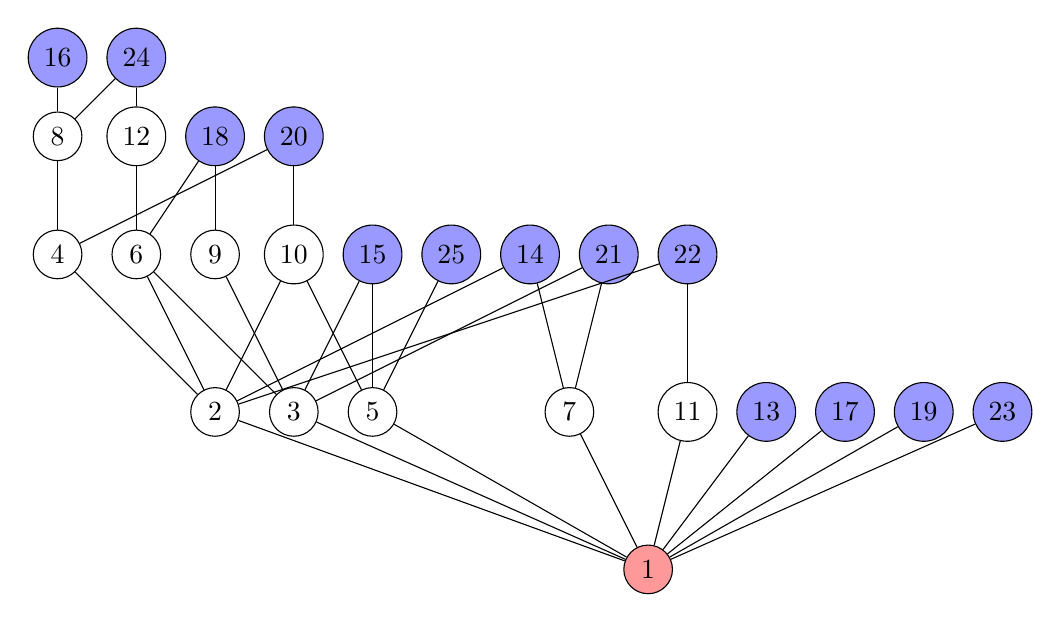
\begin{tikzpicture}
			\tikzstyle{num} = [circle, draw=black]
			\tikzstyle{minimum} = [circle, draw=black, fill=red!40]
			\tikzstyle{maximal} = [circle, draw=black, fill=blue!40]

			\node [minimum] (1) at (0,0) {1};

			\node [num, above of=1, yshift=1cm, xshift=-5.5cm] (2) {2};
			\draw (1) -- (2);

			\node [num, right of=2] (3) {3};
			\draw (1) -- (3);
			
			\node [num, right of=3, xshift=0cm] (5) {5};
			\draw (1) -- (5);
			
			\node [num, right of=5, xshift=1.5cm] (7) {7};
			\draw (1) -- (7);
			
			\node [num, right of=7, xshift=0.5cm] (11) {11};
			\draw (1) -- (11);
			
			\node [maximal, right of=11] (13) {13};
			\draw (1) -- (13);
			
			\node [maximal, right of=13] (17) {17};
			\draw (1) -- (17);
			
			\node [maximal, right of=17] (19) {19};
			\draw (1) -- (19);
			
			\node [maximal, right of=19] (23) {23};
			\draw (1) -- (23);

			\node [num, above of=2, yshift=1cm, xshift=-2cm] (4) {4};
			\draw (2) to (4);

			\node [num, above of=3, yshift=1cm, xshift=-2cm] (6) {6};
			\draw (2) -- (6);
			\draw (3) -- (6);
			
			\node [num, above of=5, yshift=1cm, xshift=-1cm] (10) {10};
			\draw (2) -- (10);
			\draw (5) -- (10);
			
			\node [maximal, above of=7, yshift=1cm, xshift=-0.5cm] (14) {14};
			\draw (2) -- (14);
			\draw (7) -- (14);
			
			\node [num, above of=4, yshift=0.5cm] (8) {8};
			\draw (4) -- (8);
			
			\node [num, right of=6] (9) {9};
			\draw (3) -- (9);
			
			\node [num, above of=6, yshift=0.5cm] (12) {12};
			\draw (6) -- (12);
			
			\node [maximal, right of=10] (15) {15};
			\draw (3) -- (15);
			\draw (5) -- (15);
			
			\node [maximal, above of=8] (16) {16};
			\draw (8) -- (16);
			
			\node [maximal, above of=9, yshift=0.5cm] (18) {18};
			\draw (6) -- (18);
			\draw (9) -- (18);
			
			\node [maximal, above of=10, yshift=0.5cm] (20) {20};
			\draw (4) -- (20);
			\draw (10) -- (20);
			
			\node [maximal, right of=14] (21) {21};
			\draw (3) -- (21);
			\draw (7) -- (21);
			
			\node [maximal, above of=11, yshift=1cm] (22) {22};
			\draw (2) -- (22);
			\draw (11) -- (22);
			
			\node [maximal, above of=12] (24) {24};
			\draw (8) -- (24);
			\draw (12) -- (24);
			
			\node [maximal, right of=15] (25) {25};
			\draw (5) -- (25);
		\end{tikzpicture}
	\end{enumerate}

	\item[8.]
	These are all the Hasse diagrams for an order relation on a set containing three elements, \(A, B, C\).
	\begin{enumerate}
		\item\adjustbox{valign=t}{
			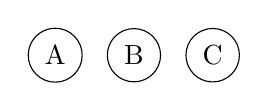
\begin{tikzpicture}
				\tikzstyle{num} = [circle, draw=black]
		
				\node [num] (A) {A};
				\node [num, right of=A] (B) {B};
				\node [num, right of=B] (C) {C};
			\end{tikzpicture}
		}
		\item\adjustbox{valign=t}{
			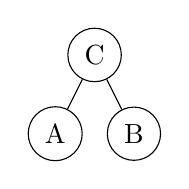
\begin{tikzpicture}
				\tikzstyle{num} = [circle, draw=black]
		
				\node [num] (A) {A};
				\node [num, right of=A] (B) {B};
				\node [num, above of=A, xshift=0.5cm] (C) {C};
				\draw (A) -- (C);
				\draw (B) -- (C);
			\end{tikzpicture}
		}
		\item\adjustbox{valign=t}{
			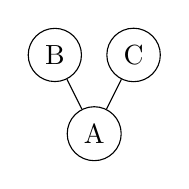
\begin{tikzpicture}
				\tikzstyle{num} = [circle, draw=black]
		
				\node [num] (A) {A};
				\node [num, above of=A, xshift=-0.5cm] (B) {B};
				\node [num, right of=B] (C) {C};
				\draw (A) -- (B);
				\draw (A) -- (C);
			\end{tikzpicture}
		}
		\item\adjustbox{valign=t}{
			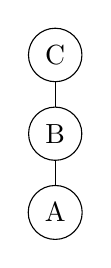
\begin{tikzpicture}
				\tikzstyle{num} = [circle, draw=black]
		
				\node [num] (A) {A};
				\node [num, above of=A] (B) {B};
				\node [num, above of=B] (C) {C};
				\draw (A) -- (B);
				\draw (B) -- (C);
			\end{tikzpicture}
		}
	\end{enumerate}
	
	\item[9.]
	\(T\) is defined as a relation on \(\mathbb{R} \times \mathbb{R}\) as follows.
	\[T = \{((a, b), (c, d)) : a^2 + b^2 \leq c^2 + d^2\}\]
	\begin{enumerate}
		\item % a
		\(T\) is reflexive, since \(a^2 + b^2 \leq a^2 + b^2\).

		\item % b
		\(T\) is antisymmetric since if \(a^2 + b^2 < c^2 + d^2\), then \(c^2 + d^2 \nless a^2 + b^2\).

		\item % c
		\(T\) is transitive since if \(a^2 + b^2 < c^2 + d^2\), and \(c^2 + d^2 < e^2 + f^2\), then \(a^2 + b^2 < e^2 + f^2\).
	\end{enumerate}
	Therefore \(T\) is an order relation.

	\item[10.]
	\(S\) is defined as a relation on \(\mathbb{N} \times \mathbb{N}\) as follows.
	\[S = \{((x, y), (m, n)) : x|m \land y|n\}\]
	\begin{enumerate}
		\item % a
		\(S\) is reflexive since every natural number divides itself.

		\item % b
		\(S\) is antisymmetric since if \(a \neq b\) and \(a|b\) then \(b \nmid a\).

		\item % c
		\(S\) is transitive since if \(a|b\) and \(b|c\), then \(a|c\). Another way to think about this is as follows. If \(a|b\) then \(b = a \times k_1\), where \(k_1 \in \mathbb{N}\). If \(b|c\), then \(c = b \times k_2\), where \(k_2 \in \mathbb{N}\). Therefore \(c = a \times k_1 \times k_2\), so this all implies that \(a\) must divide \(c\).
	\end{enumerate}
	Therefore \(S\) is an order relation.

	\item[11.]
	\begin{enumerate}
		\item % a
		Since \(R\) is an order relation, it must have the antisymmetric property, which states that \(\forall x, y \in A\), if \(xRy\) and \(yRx\), then it must be that \(x = y\). Therefore, since all elements \((x, y) \in S\) satisfy both \(xRy\) and \(yRx\), all element in \(S\) must be of the form \((x, x)\).

		\(S\) is clearly reflexive, as we just explained. It is also symmetric, si
		\(S\) is clearly reflexive, as we just explained. It is also symmetric, si
		\(S\) is clearly reflexive, as we just explained. It is also symmetric, since elements can only be related to themselves. And for the same reason \(S\) must also be transitive.
		\[S = R \cap R^{-1}\]

		\item % b
		\(S\) is not necessarily an equivalence relation, since we are not guaranteed that it is transitive. For example, if we have \(R\) such that \(aRc\) and \(bRc\) but \(a {\centernot{R}} b\) and \(b {\centernot{R}} a\), then \(S\) must be such that \(aSc\), \(bSc\), \(cSa\), and \(cSb\), but we will not have \(aSb\) or \(bSa\).
		\[S = R \cup R^{-1}\]

		\item % c
		\(S\) not an equivalence relation on \(A\) since it is not always transitive. Let \(a, b, c, d, e\) be elements of \(A\). If we have \(R\) such that \(aRd\) and \(bRd\), and we also have \(bRe\) and \(cRe\), but \(\nexists f \in A\) such that \(aRf\) and \(cRf\), then we have a case where \(aSb\) and \(bSd\) but \(a{\centernot{S}}c\).

		An example where this is the case is as follows. Let \(A\) and \(R\) be defined as in question 7(c).
		\begin{gather*}
			A = \{x \in \mathbb{N}_1 : x \leq 25\} \\
			R = \{(a, b) \in A \times A : a|b\}
		\end{gather*}

		Here we have \(4R24\) and \(6R24\), so \(4S6\). We also have \(6R18\) and \(9R18\), so \(6R9\). But there is no element in \(A\) such that both 4 and 9 are related to it. Therefore \(4{\centernot{S}}9\).
	\end{enumerate}

	\item[13.]
	Let \(R\) and \(S\) be order relations on a set \(A\). 
	\begin{enumerate}
		\item[(a)]
		\(R \cap S\) is an order relation on \(A\).
		\begin{enumerate}
			\item % i
			In order for \(R \cap S\) to be reflexive, it must contain every element \((a, a) \in A \times A\). But we know that both \(R\) and \(S\) are reflexive, so they both contain all of those elements, therefore \(R \cap S\) also contains them, so \(R \cap S\) is reflexive.

			\item % ii
			In order for \(R \cap S\) to be antisymmetric, it must be true that if it contains an element \((a, b)\) such that \(a \neq b\), then it does not contain the element \((b, a)\). We know, however, that if \(R \cap S\) contains \((a, b)\), then both \(R\) and \(S\) contain it as well. And since both \(R\) and \(S\) are antisymmetric, we also know that neither of them can contain \((b, a)\). Therefore neither does \(R \cap S\), so it is antisymmetric.

			\item % iii
			In order for \(R \cap S\) to be transitive, it must be true that if it contains two elements \((a, b)\) and \((b, c)\), then it must contain the element \((a, c)\). We also know that if \(R \cap S\) contains both \((a, b)\) and \((b, c)\), then both \(R\) and \(S\) contain them as well. And since both \(R\) and \(S\) are transitive, we also know that both of them must contain \((a, c)\). Therefore so does \(R \cap S\), so it is transitive.
		\end{enumerate}

		\item[(d)]
		\(R^{-1}\) is an order relation on \(A\).
		\begin{enumerate}
			\item % i
			In order for \(R^{-1}\) to be reflexive, it must contain every element \((a, a) \in A \times A\). But we know that \(R\) is reflexive, so it contains all of those elements, therefore \(R^{-1}\) also contains them because the inverse of \((a, a)\) is also \((a, a)\), so \(R^{-1}\) is reflexive.

			\item % ii
			In order for \(R^{-1}\) to be antisymmetric, it must be true that if it contains an element \((a, b)\) such that \(a \neq b\), then it does not contain the element \((b, a)\). We know, however, that if \(R^{-1}\) contains \((a, b)\), then \(R\) contains \((b, a)\). And since \(R\) is antisymmetric, we also know that it cannot contain \((a, b)\). Therefore \(R^{-1}\) does not contain \((b, a)\), so it is antisymmetric.

			\item % iii
			In order for \(R^{-1}\) to be transitive, it must be true that if it contains two elements \((a, b)\) and \((b, c)\), then it must contain the element \((a, c)\). We also know that if \(R^{-1}\) contains both \((a, b)\) and \((b, c)\), then \(R\) must contain \(c, b\) and \(b, a\). And since \(R\) is transitive, we also know that it must contain \((c, a)\). Therefore \(R^{-1}\) contains \((a, c)\), so it is transitive.
		\end{enumerate}
	\end{enumerate}

	\item[16]
	\begin{enumerate}
		\item[(b)]
		\(R\) is reflexive and transitive. If \(R\) is \textit{not} an order relation, it must be that \(R\) is not antisymmetric. Meaning, it must contain two elements of the form \((a, b)\) and \((b, a)\) such that \(a \neq b\). Therefore \(S\) would also contain an element \((a, b)\) such that \(a \neq b\), so \(S\) would not be the identity relation on \(X\).

		However if \(R\) \textit{is} an order relation, then it must be antisymmetric, so it does not contain any two elements \(a, b\) and \(b, a\) such that \(a \neq b\). Therefore there is no element \((a, b) \in S\) such that \(a \neq b\). Furthermore, since \(R\) is reflexive, it must contain the element \((a, a)\) for all \(a \in X\), which means that \(S\) would also contain those. Therefore \(S\) must be the identity relation on \(X\).
	\end{enumerate}

	\item[17.]
	\begin{enumerate}
		\item % a
		\begin{enumerate}
			\item % i
			\(S\) is reflexive, since every set is a subset of itself, and since they contain the exact same elements they have the same \(Min\).

			\item % ii
			\(S\) is antisymmetric, because if you have two sets \(A\) and \(B\), the only way that they can both be subsets of each other is if they are the same set.

			\item % iii
			\(S\) is transitive, since `is a subset of' and `equals' are both transitive relations. So since every two sets related by \(S\) must satisfy those two relations, \(S\) must be transitive.
		\end{enumerate}

		\item\adjustbox{valign=t}{
			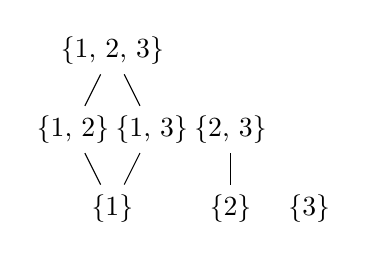
\begin{tikzpicture}
				\node (1) at (0,0) {\{1\}};
				\node [right of=1, xshift=0.5cm] (2) {\{2\}};
				\node [right of=2] (3) {\{3\}};

				\node [above of=1, xshift=-0.5cm] (1_2) {\{1, 2\}};
				\draw (1) to (1_2);

				\node [right of=1_2] (1_3) {\{1, 3\}};
				\draw (1) to (1_3);

				\node [above of=2] (2_3) {\{2, 3\}};
				\draw (2) to (2_3);

				\node [above of=1_2, xshift=0.5cm] (1_2_3) {\{1, 2, 3\}};
				\draw (1_2) to (1_2_3);
				\draw (1_3) to (1_2_3);
			\end{tikzpicture}
		}
	\end{enumerate}

	\item[19.]
	\begin{enumerate}
		\item % a
		There are six equivalence classes in \(\approx\).

		\item % b
		\({^5}\text{C}_2 = {^5}\text{C}_3 = 10\)
	\end{enumerate}

	\item[24.]  
	\begin{enumerate}
		\item % a
		\begin{enumerate}
			\item % i
			\(R\) is not an order relation, since it is not antisymmetric. If two \(X\) and \(Y\) are two distinct subsets of \(A\) such that they both have the same max, they will both be related to each other. For example, \(\{1, 3\}R\{2, 3\}\) and \(\{2, 3\}R\{1, 3\}\).

			\item % ii
			\begin{gather*}
				Max(\{2, 5, 7\}) = 7 \\
				Max(\{2, 3, 4, 5, 7\}) = 7 \\
				\Rightarrow \{2, 3, 4, 5, 7\}\ R\ \{2, 5, 7\} \\
				\Rightarrow \{2, 5, 7\}\ R^{-1}\ \{2, 3, 4, 5, 7\}
			\end{gather*}
		\end{enumerate}

		\item % b
		\begin{enumerate}
			\item % i
			\(R\) is not an order relation since it is not reflexive.
			\[|X| = |X| \quad \Rightarrow \quad |X| \nless |X| \quad \Rightarrow \quad X{\centernot{R}}X\]

			\item % ii
			\begin{gather*}
				\{2, 3, 7\}\ R\ \{1, 2, 3, 4\} \\
				\{1, 2, 3, 4\}\ R\ \{1, 3, 4, 5, 8\} \\
				\Rightarrow \{2, 3, 7\}\ R \circ R\ \{1, 3, 4, 5, 8\} \\
			\end{gather*}
		\end{enumerate}
	\end{enumerate}
\end{enumerate}
	
\end{document}
